\documentclass{standalone}
\usepackage{tikz}
\begin{document}
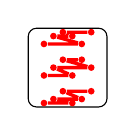
\begin{tikzpicture}[scale=1.0]
  % draw rounded cell boxes
  \draw[rounded corners=3pt] (0,0) rectangle (1,1);
  \node[circle, fill=red, inner sep=0.03cm] (obs2443273672880_pt0) at (0.2,0.05) {};
  \node[circle, fill=red, inner sep=0.03cm] (obs2443273672880_pt1) at (0.32,0.1) {};
  \node[circle, fill=red, inner sep=0.03cm] (obs2443273672880_pt2) at (0.44,0.2) {};
  \node[circle, fill=red, inner sep=0.03cm] (obs2443273672880_pt3) at (0.56,0.05) {};
  \node[circle, fill=red, inner sep=0.03cm] (obs2443273672880_pt4) at (0.6799999999999999,0.1) {};
  \node[circle, fill=red, inner sep=0.03cm] (obs2443273672880_pt5) at (0.8,0.2) {};
  \draw[red, line width=1.2pt] (obs2443273672880_pt0) -- (obs2443273672880_pt3) -- (obs2443273672880_pt1) -- (obs2443273672880_pt4) -- (obs2443273672880_pt2) -- (obs2443273672880_pt5);
  \node[circle, fill=red, inner sep=0.03cm] (obs2443273052112_pt0) at (0.2,0.4) {};
  \node[circle, fill=red, inner sep=0.03cm] (obs2443273052112_pt1) at (0.32,0.5) {};
  \node[circle, fill=red, inner sep=0.03cm] (obs2443273052112_pt2) at (0.44,0.6000000000000001) {};
  \node[circle, fill=red, inner sep=0.03cm] (obs2443273052112_pt3) at (0.56,0.4) {};
  \node[circle, fill=red, inner sep=0.03cm] (obs2443273052112_pt4) at (0.6799999999999999,0.6000000000000001) {};
  \node[circle, fill=red, inner sep=0.03cm] (obs2443273052112_pt5) at (0.8,0.5) {};
  \draw[red, line width=1.2pt] (obs2443273052112_pt0) -- (obs2443273052112_pt3) -- (obs2443273052112_pt1) -- (obs2443273052112_pt5) -- (obs2443273052112_pt2) -- (obs2443273052112_pt4);
  \node[circle, fill=red, inner sep=0.03cm] (obs2443273435856_pt0) at (0.2,0.8) {};
  \node[circle, fill=red, inner sep=0.03cm] (obs2443273435856_pt1) at (0.32,0.9) {};
  \node[circle, fill=red, inner sep=0.03cm] (obs2443273435856_pt2) at (0.44,0.95) {};
  \node[circle, fill=red, inner sep=0.03cm] (obs2443273435856_pt3) at (0.56,0.9) {};
  \node[circle, fill=red, inner sep=0.03cm] (obs2443273435856_pt4) at (0.6799999999999999,0.8) {};
  \node[circle, fill=red, inner sep=0.03cm] (obs2443273435856_pt5) at (0.8,0.95) {};
  \draw[red, line width=1.2pt] (obs2443273435856_pt0) -- (obs2443273435856_pt4) -- (obs2443273435856_pt1) -- (obs2443273435856_pt3) -- (obs2443273435856_pt2) -- (obs2443273435856_pt5);
\end{tikzpicture}
\end{document}